\documentclass[tikz,border=5pt]{standalone}
\usepackage{tikz}
\usepackage{pgfplots}
\usepgfplotslibrary{groupplots}
\pgfplotsset{compat=1.18}
% sha256: ba0afe06f43b4dc71b98f5c991e67e698722cd6018c9ae6b2bc6a94a1d16fdda
\definecolor{p06color0}{HTML}{0072B2}
\definecolor{p06color1}{HTML}{D55E00}
\definecolor{p06color2}{HTML}{009E73}
\begin{document}
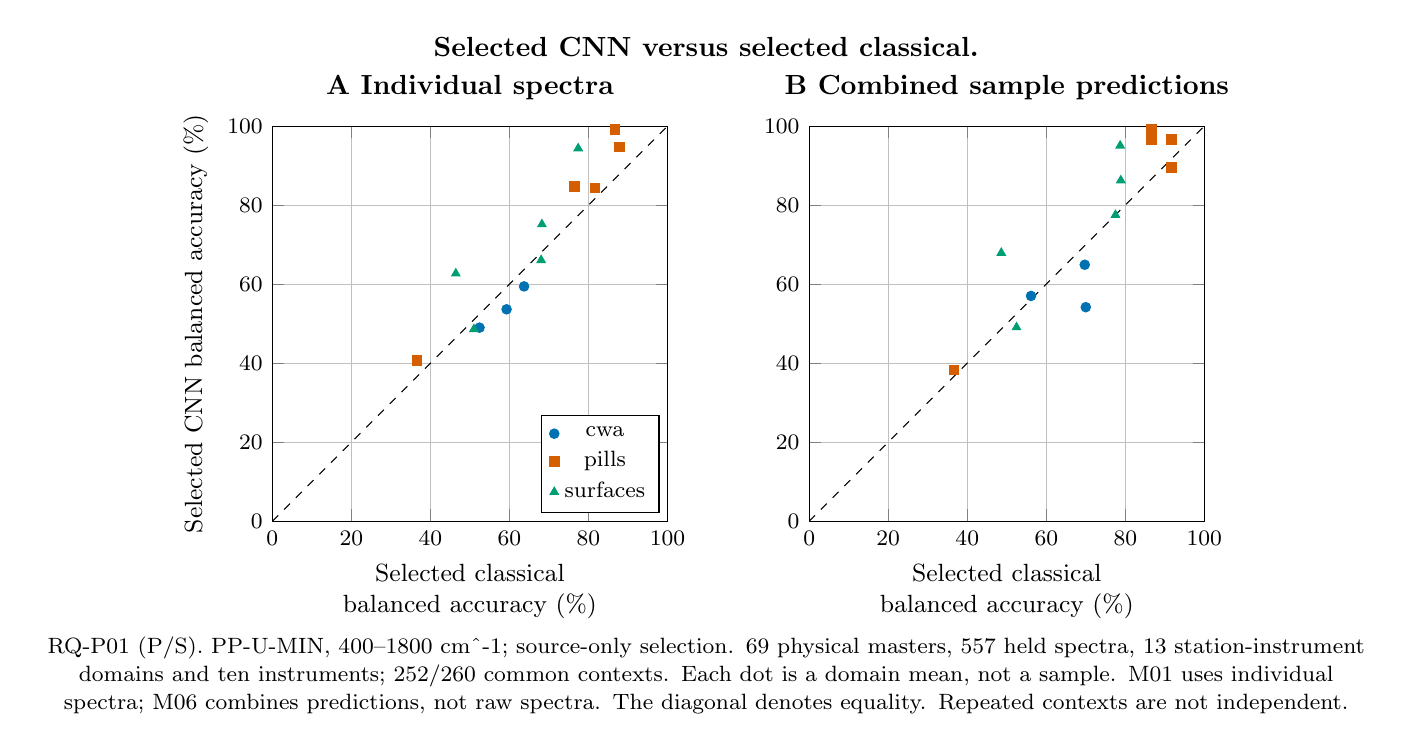
\begin{tikzpicture}
\begin{groupplot}[group style={group size=2 by 1, horizontal sep=1.8cm},
width=6.6cm,
height=6.6cm,
xmin=0, xmax=100, ymin=0, ymax=100,
xlabel={Selected classical\\balanced accuracy (\%)},
xlabel style={font=\fontsize{9}{11}\selectfont, color=black, align=center},
ylabel={Selected CNN balanced accuracy (\%)},
ylabel style={font=\fontsize{9}{11}\selectfont, color=black},
tick label style={font=\fontsize{8}{10}\selectfont, color=black},
title style={font=\bfseries\fontsize{10}{12}\selectfont, color=black},
grid=both,
axis equal]
\nextgroupplot[title={A Individual spectra}, legend style={at={(0.98,0.02)},anchor=south east,draw=black,fill=white,font=\fontsize{8}{10}\selectfont}]
\addplot[forget plot, black, thin, dashed] coordinates {(0,0) (100,100)};
\addplot[only marks, mark=*, mark size=1.7pt, color=p06color0] coordinates {(59.2799422799423,53.6328763828764) (52.4408242829295,48.9933166248956) (63.7134502923977,59.4277360066834)};
\addlegendentry{cwa}
\addplot[only marks, mark=square*, mark size=1.7pt, color=p06color1] coordinates {(76.5,84.75) (87.9166666666667,94.7222222222222) (36.6666666666667,40.6369047619048) (81.609126984127,84.3313492063492) (86.6666666666667,99.1666666666667)};
\addlegendentry{pills}
\addplot[only marks, mark=triangle*, mark size=1.7pt, color=p06color2] coordinates {(51.0185185185185,48.6111111111111) (46.4384920634921,62.6944444444444) (77.4074074074074,94.3650793650794) (68.2275132275132,75.1410934744268) (68.0358946608947,66.0728715728716)};
\addlegendentry{surfaces}
\nextgroupplot[title={B Combined sample predictions}, ylabel={}]
\addplot[forget plot, black, thin, dashed] coordinates {(0,0) (100,100)};
\addplot[only marks, mark=*, mark size=1.7pt, color=p06color0] coordinates {(70,54.1666666666667) (56.140350877193,57.0175438596491) (69.7368421052632,64.9122807017544)};
\addplot[only marks, mark=square*, mark size=1.7pt, color=p06color1] coordinates {(91.6666666666667,89.5833333333333) (91.6666666666667,96.6666666666667) (36.6666666666667,38.3333333333333) (86.6666666666667,96.6666666666667) (86.6666666666667,99.1666666666667)};
\addplot[only marks, mark=triangle*, mark size=1.7pt, color=p06color2] coordinates {(52.4691358024691,49.0740740740741) (48.6111111111111,67.9166666666667) (78.7037037037037,95.0617283950617) (78.858024691358,86.2654320987654) (77.5,77.5)};
\end{groupplot}
\node[anchor=south, font=\bfseries\fontsize{10}{12}\selectfont] at (current bounding box.north) {Selected CNN versus selected classical.};
\node[anchor=north, text width=17cm, align=center, font=\fontsize{8}{10}\selectfont] at (current bounding box.south) {RQ-P01 (P/S). PP-U-MIN, 400–1800 cm\textasciicircum{}-1; source-only selection. 69 physical masters, 557 held spectra, 13 station-instrument domains and ten instruments; 252/260 common contexts. Each dot is a domain mean, not a sample. M01 uses individual spectra; M06 combines predictions, not raw spectra. The diagonal denotes equality. Repeated contexts are not independent.};
\end{tikzpicture}
\end{document}
